 \documentclass[11pt]{amsart}

\usepackage[nocompress]{cite} % puts in-text citation numbers in order

\usepackage[normalem]{ulem}
%\usepackage{subfloat}
\usepackage{subfigure}
\usepackage{caption}
%\usepackage{subcaption}
\usepackage{amsaddr}
\usepackage{color}
%\usepackage{enumitem}
\usepackage{enumerate}
%\usepackage{natbib}
\usepackage{bbm}
\usepackage[mathscr]{eucal}
\usepackage{verbatim}
\usepackage{hyperref}
\usepackage{graphicx}
\usepackage{mathtools}
\usepackage[margin=1in]{geometry}
\usepackage{amsmath}
\usepackage{amssymb}
\newcommand*{\QEDB}{\hfill\ensuremath{\square}}%

\newcommand{\foot}[1]{\mbox{}\marginpar{\raggedleft\hspace{0pt}\tiny #1}}
%\newcommand{\foot}[1]{}
\newcommand{\NN}{\mathbb{N}}
\newcommand{\ZZ}{\mathbb{Z}}
\newcommand{\sign}{{\rm sign}}
\newtheorem{definition}{Definition}[section]
\newtheorem{notation}{Notation}[section]
\newtheorem{theorem}{Theorem}[section]
\newtheorem{lemma}[theorem]{Lemma}
\newtheorem{proposition}[theorem]{Proposition}
\newtheorem{corollary}[theorem]{Corollary}
\newtheorem{thma}{Theorem}
\renewcommand{\thethma}{\Alph{thma}}
\theoremstyle{remark}
\newtheorem*{remark}{Remark}


\numberwithin{equation}{section}
\newcommand{\reals}{\mathbb{R}}
\newcommand{\ones}{\mathbf{1}}
\DeclareMathOperator*{\argmin}{arg\,min}

%\usepackage{authblk}
%\usepackage{caption}
%\usepackage{subcaption}

\def\presuper#1#2%
  {\mathop{}%
   \mathopen{\vphantom{#2}}^{#1}%
   \kern-\scriptspace%
   #2}

\DeclareMathOperator*{\IGP}{\presuper{IGP}{\mathit{A}}}
\DeclareMathOperator*{\Tri}{\presuper{Tri}{\mathit{A}}}
\DeclareMathOperator*{\MRS}{{\rm MRS}}
\DeclareMathOperator*{\SSS}{{\rm SS}}
%\DeclareMathOperator*{\NS}{NS}
\newcommand{\NS}{NS}

\newcommand{\mn}{\color{blue}}

\newcommand{\themethod}{containment min hash}
\DeclareMathOperator*{\Jac}{{\rm Jac}}


% % % % % % % % % % % % % % % %
% Potential reviewers:
% 

% % % % % % % % % % % % % % % % % % % % % % % % % % % % % % % % % % % % % %

\begin{document}



\title[Improving Min Hash]{Improving Min Hash for Metagenomic Taxonomic Profiling} %Inside the square brackets is the running head


\author{Hooman Zabeti${}^{1}$, David Koslicki${}^{1*}$}
\address{${}^1$ Mathematics Department, Oregon State University, Corvallis, OR.}
\thanks{${}^*$ Corresponding Author: \url{david.koslicki@math.oregonstate.edu}}





\date{\today}
\begin{abstract}
Abstract here.  \\\\
\smallskip
\noindent \textsc{Keywords}: \emph{Min hash, k-mins sketch, metagenomics, taxonomic profiling, taxonomic classification, Jaccard index, containment}.
\end{abstract}
\maketitle


\section{Introduction}
\begin{enumerate}
\item Min hash recently has been used to great success on biological data
\item Mash, Titus' sourmash
\item originally designed for sets of relatively similar size and appreciable intersection size
\item metagenomic taxonomic profiling the setup is different: many relatively small database entries, one very large metagenomic sample, very small intersection sizes in general
\item we modify the min hash paradigm to this particular situation so it can handle a sample of much greater size than the reference database entries.
\end{enumerate}





\section{Methods}
Definitions, derivation of mathematical results here.
\subsection{Definitions}
\begin{enumerate}
\item Definitions of database entries, query sample, k-mer size, note size disparity
\item define classic min hash (k-independent version and k-mins version)
\item define the containment approach
\end{enumerate}
\subsection{Min Hash via containment}
\label{section:ChernoffBounds}
\subsection{Time and space complexity}
\begin{enumerate}
\item Chernoff bound estimates
\item comparison of number of hashes required for same accuracy
\item time complexity
\item space complexity (all with examples of the numbers in practice).
\end{enumerate}


\section{Results}
In this section, we compare classic min hash to the proposed method.
\subsection{Synthetic data}
\label{section:SyntheticData}
Here we illustrate the improved accuracy of \themethod over classical min hash in estimating the Jaccard index. To that end, we generated two random strings $w_A$ and $w_B$ on the alphabet $\{A,C,T,G\}$. We set $|w_A|= 10,000$ and $|w_B| = 15$ to simulate the situation of interest where one wishes to estimate the Jaccard index of two sets of very different size. We then appended a common string $w_C$ of increasing length to each of $w_A$ and $w_B$ so that $\Jac_k(w_Aw_C, w_Bw_C)$ ranges between 0 and 1. We picked the $k$-mer size of $11$ and utilized a signature size of 100. Figure \ref{fig:TrueVsEstimate} depicts the comparison of \themethod with the classical min hash Jaccard estimate on this data and effectively illustrates the results in section \ref{section:ChernoffBounds} which proved that the containment approach has a higher probably of being closer to the true Jaccard than the classic approach. The mean and variance of the classic min hash approach on this data was \input{SyntheticDataClassic.txt} while using the containment approach, this improved to \input{SyntheticDataContainment.txt}.


\begin{figure}[!h]%
\begin{center}
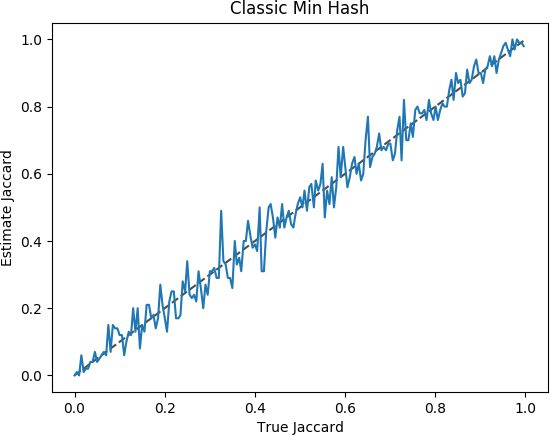
\includegraphics[width=3.25in,trim={0 0 0 0in},clip]{Figs/TrueVsEstimate.png}%
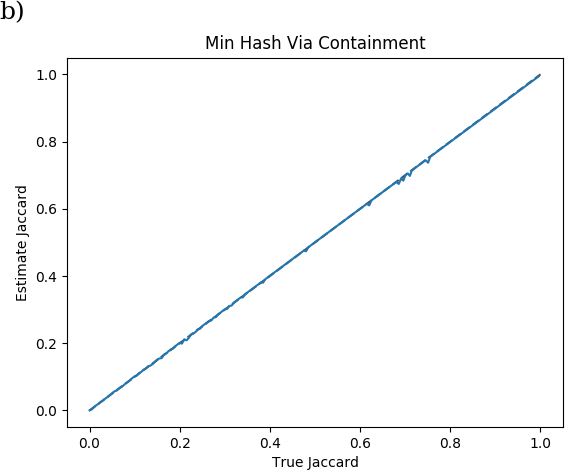
\includegraphics[width=3.25in,trim={0 0 0 0in},clip]{Figs/ContainmentTrueVsEstimate.png}
\end{center}
\caption{Comparison of \themethod to the classical min hash estimate of the Jaccard index on synthetic data. Each method utilized the 100 smallest hashes of the murmer3 hash function on the $11$-mers of two randomly generated strings with sizes 10,000 and 15 respectively after appending a common substring of increasing size. a) Classical min hash estimate of the Jaccard index. b) The proposed \themethod on the same data.}
\label{fig:TrueVsEstimate}%
\end{figure}


\subsection{Simulated biological data}
\subsection{Real biological data}

\section{Discussion}


\clearpage
\bibliography{library}{}
\bibliographystyle{abbrv}

\end{document}

